% !TeX root = incremental_SS_Translation.tex
\chapter{Kalpasthāna: Introduction}

\section{The Sequence of Chapters}
\label{kalpa-chapter-sequence}
The Nepalese version of the \SS\ reverses the sequence of chapters 6 and 7.  

\begin{table}[h]
    \centering
     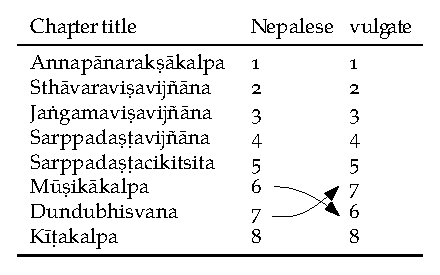
\includegraphics[width=0.65\linewidth]{chapters/media/kalpa}
%    \begin{tabular}{lll}
%    \emph{Chapter title} & \emph{Nepalese} & \emph{vulgate}   \\
%    \toprule
%      Annapānarakṣākalpa   &  1 &  1 \\
%     Sthāvaraviṣavijñāna & 2 &  2\\
%     Jaṅgamaviṣavijñāna &  3 & 3 \\
%     Sarppadaṣṭavijñāna & 4  &  4 \\
%     Sarppadaṣṭacikitsita & 5 & 5 \\
%     Mūṣikākalpa &  {6} & \textbf{7} \\
%     Dundubhisvana & {7} & \textbf{6} \\
%     Kīṭakalpa & 8 & 8 \\
%    \bottomrule  
%    \end{tabular}
\end{table}

% TODO: \usepackage{graphicx} required
%\begin{figure}
%    \centering
%    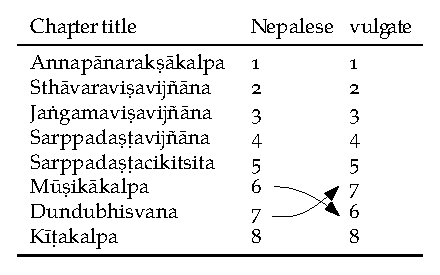
\includegraphics[width=0.65\linewidth]{chapters/media/kalpa}
%    \caption{}
%    \label{fig:kalpa}
%\end{figure}

\noindent
This difference in sequence does not have an immediately obvious 
significance, but it appears to be the most original known sequence of 
chapters, since it was already known to Jejjaṭa.\footnote{See note 
\ref{dalhana-rat-sequence} below.}

\section{The Spread of Indian Toxicological Lore to Medieval Islamic 
Authors}

\citet[Introduction]{leve-1966} on 
\begin{itemize}
    \item tr. of the \SS\ under the Barmakids (Pramukhas) in 
    eighth-ninth-century Baghdad.
    \begin{quote}
        Much more important is the fact
        that Mankah is known as the translator of the Susruta
        samhita, a huge medical compendium, for Yahya b.
        Khalid. Ibn abi Usaibi'a (1203/4-1270) also discusses
        Mankah as an important Indian physician. Al-Jaiz
        (d. 868/9) knew of Mankah.'
        \ldots
        
        Yahya ibn Khalid, a Barmecide, was famous in his
        day in the field of science. In ibn al-Nadim, it is
        related that Yah.ya sent a scholar to India to study
        Indian drugs and religion, and brought Indian physi-
        cians and philosophers westward so that he might learn
        from them.
        Caliph al-Ma'mfin  also was interested in the sci-
        ences and so brought many scientists to his court from
        Jundishapfir where there were not only Greek men of
        science but also Indians who had brought their science
        and wisdom.
        \footnote{\cite[6]{leve-1966}}
    \end{quote}
    
    \item ibn Wahshiya's Book on Poisons (ca. 950). 
    \begin{quote}
        Not much is known of Shanaq himself. However,
        what is one of the earliest mentions of him is made in
        ibn Wahshiya's Book on Poisons (ca. 950). He refers
        to Shanaq's book as great and important. This state-
        ment is attested to by the fact that much of Shanaq's
        work was used by ibn Wahshiya. It was not, however,
        a base upon which the latter's work was built, as
        Strauss has claimed.
    \end{quote}
    \item The Poison book of Cāṇakya. 
\end{itemize}

The Poison Book of Maimonides:
\begin{itemize}
    \item \fullcite[]{rosn-1968}.  Written in approximately July 1198 
    at the request of his patron, al-Qadi al-Fadil (1135--1200) who 
    served in Cairo under the Fatimid and Ayyubid 
    administrations.\foocite[31]{krae-2005} 
\end{itemize}em 
